\subsection{Grandmother number-units}
To succeessfully perform subject-verb agreement, the LSTM network should encode and store the grammatical number of the subject up to one step before the verb, when prediction of the verb form (singular or plural) occurs. In some cases, this may be quite challenging, in particular, in the case of a long-range dependency between subject and verb, and when another noun with an opposite number appears before the verb (cite and cite). This section explores the underlying mechanism that enables the network to encode and store number information in various syntactic constructions, inculding those with an such interferring nouns. Section 5.1.1 describes an ablation study, which reveals \textit{long-range number units (LR-number units)} that can carry number information from subject to verb across an interfering noun. Then, section 5.1.2 describes in details the gating and state dynamics of the identified LR-number units during the processing of sentences with long-range dependency between subject and verb. Finally, section 5.1.3 explores the structure of the efferent weights of LG-number units. These efferent weights propagate grammatical-number information to the output layer, allowing for the prediction of the proper verb form (singular or plural). 

\subsubsection{Ablation study}
Generally, number information may be stored in the network in either a local, sparse, or a distributed way, dpending on the fraction of active units that carry this information. We hypothesized that if the network uses a local or sparse coding, meaning that there's a small set of units that encode number information, then ablating these units would lead to a drastic decrease in perofrmance on the NA-task, compared to when ablating other units. To test this, we conducted ablation experiments in which each time a single unit of the network is ablated and the resulting model is then evaluated on several NA-tasks. Each NA-task contained sentences with a fixed syntactic structure and was composed of several \textit{conditions} according to the possible values of grammatical numbers of its noun(s). For example, the first task was to predict the correct verb form in sentences with the following strcture: "Det Noun Verb", such as "The boy runs". This task had two conditions, corresponding to the two possible assignments of grammatical number to the main noun. Another task was to predict the correct verb form in sentences of the form: "Det Noun-1 P Det Noun-1 Verb", such as "The boy behind the girls jumps". This task had four conditions, corresponding to the four possible assignments of grammatical number to noun-1 and noun-2. Finally, we also evaluated the ablated model on the Linzen task (section 3.1). Tables 1 \& 2 summarize the results of all ablation experiments. 


\begin{tabular}{ |p{3cm}||p{3cm}|p{3cm}|}
 \hline
 & N1-singular & N1-plural \\
 \hline
 \hline
 Simple & 100\% & 100\% \\
 Single-adv & 100\% & 99.56\% \\
 Two-adv & 99.78\% & 99\% \\
 name-PP & 98.89\% & 66.78\% \\
 adv-conj & 98.83\% & 99.67\% \\ 
 \hline
\end{tabular}

\begin{tabular}{ |p{3cm}||p{3cm}|p{3cm}|p{3cm}|p{3cm}|}
 \hline
 & SS & SP & PS & PP\\
\hline
\hline
 with-PP & 97.5\% & 88.5\% 93.1\% & &  \\
 subjrel & & & & \\
 objrel & & & & \\
 \hline
\end{tabular}



Section 5.1.1 describes the results of this study, showing that a significant descrease in task performance is indeed observed for only a small set of units, therefore suggesting a local code carried by what we call \textit{long-range number units (LR-number units)}. We next hypothesized that the storage of number information in these units should be apparent in their gates and state dynamics. For example, to carry number information from the subject to the verb, the forget-gate activity is likely to be close to one, whereas input-gate activity is likely to be non-zero only during the presentation time of the subject (Figure 1B). To explore this, we visualized gates and state dynamics of LR-number units during the processing of well-controlled sets of stimuli (section 3.1) - Section 5.1.2 summarizes these findings. Finally, to predict the proper verb form, number information should be projected from number units to the output layer. Section 5.1.3 explores the structure of the efferent weights of the number units. 



\subsubsection{Visualizing unit dynamics}
In particular, to carry number information from the subject to the verb, the forget gate of number units should be set to one during the entire period that separates them. 


\begin{figure}[t]
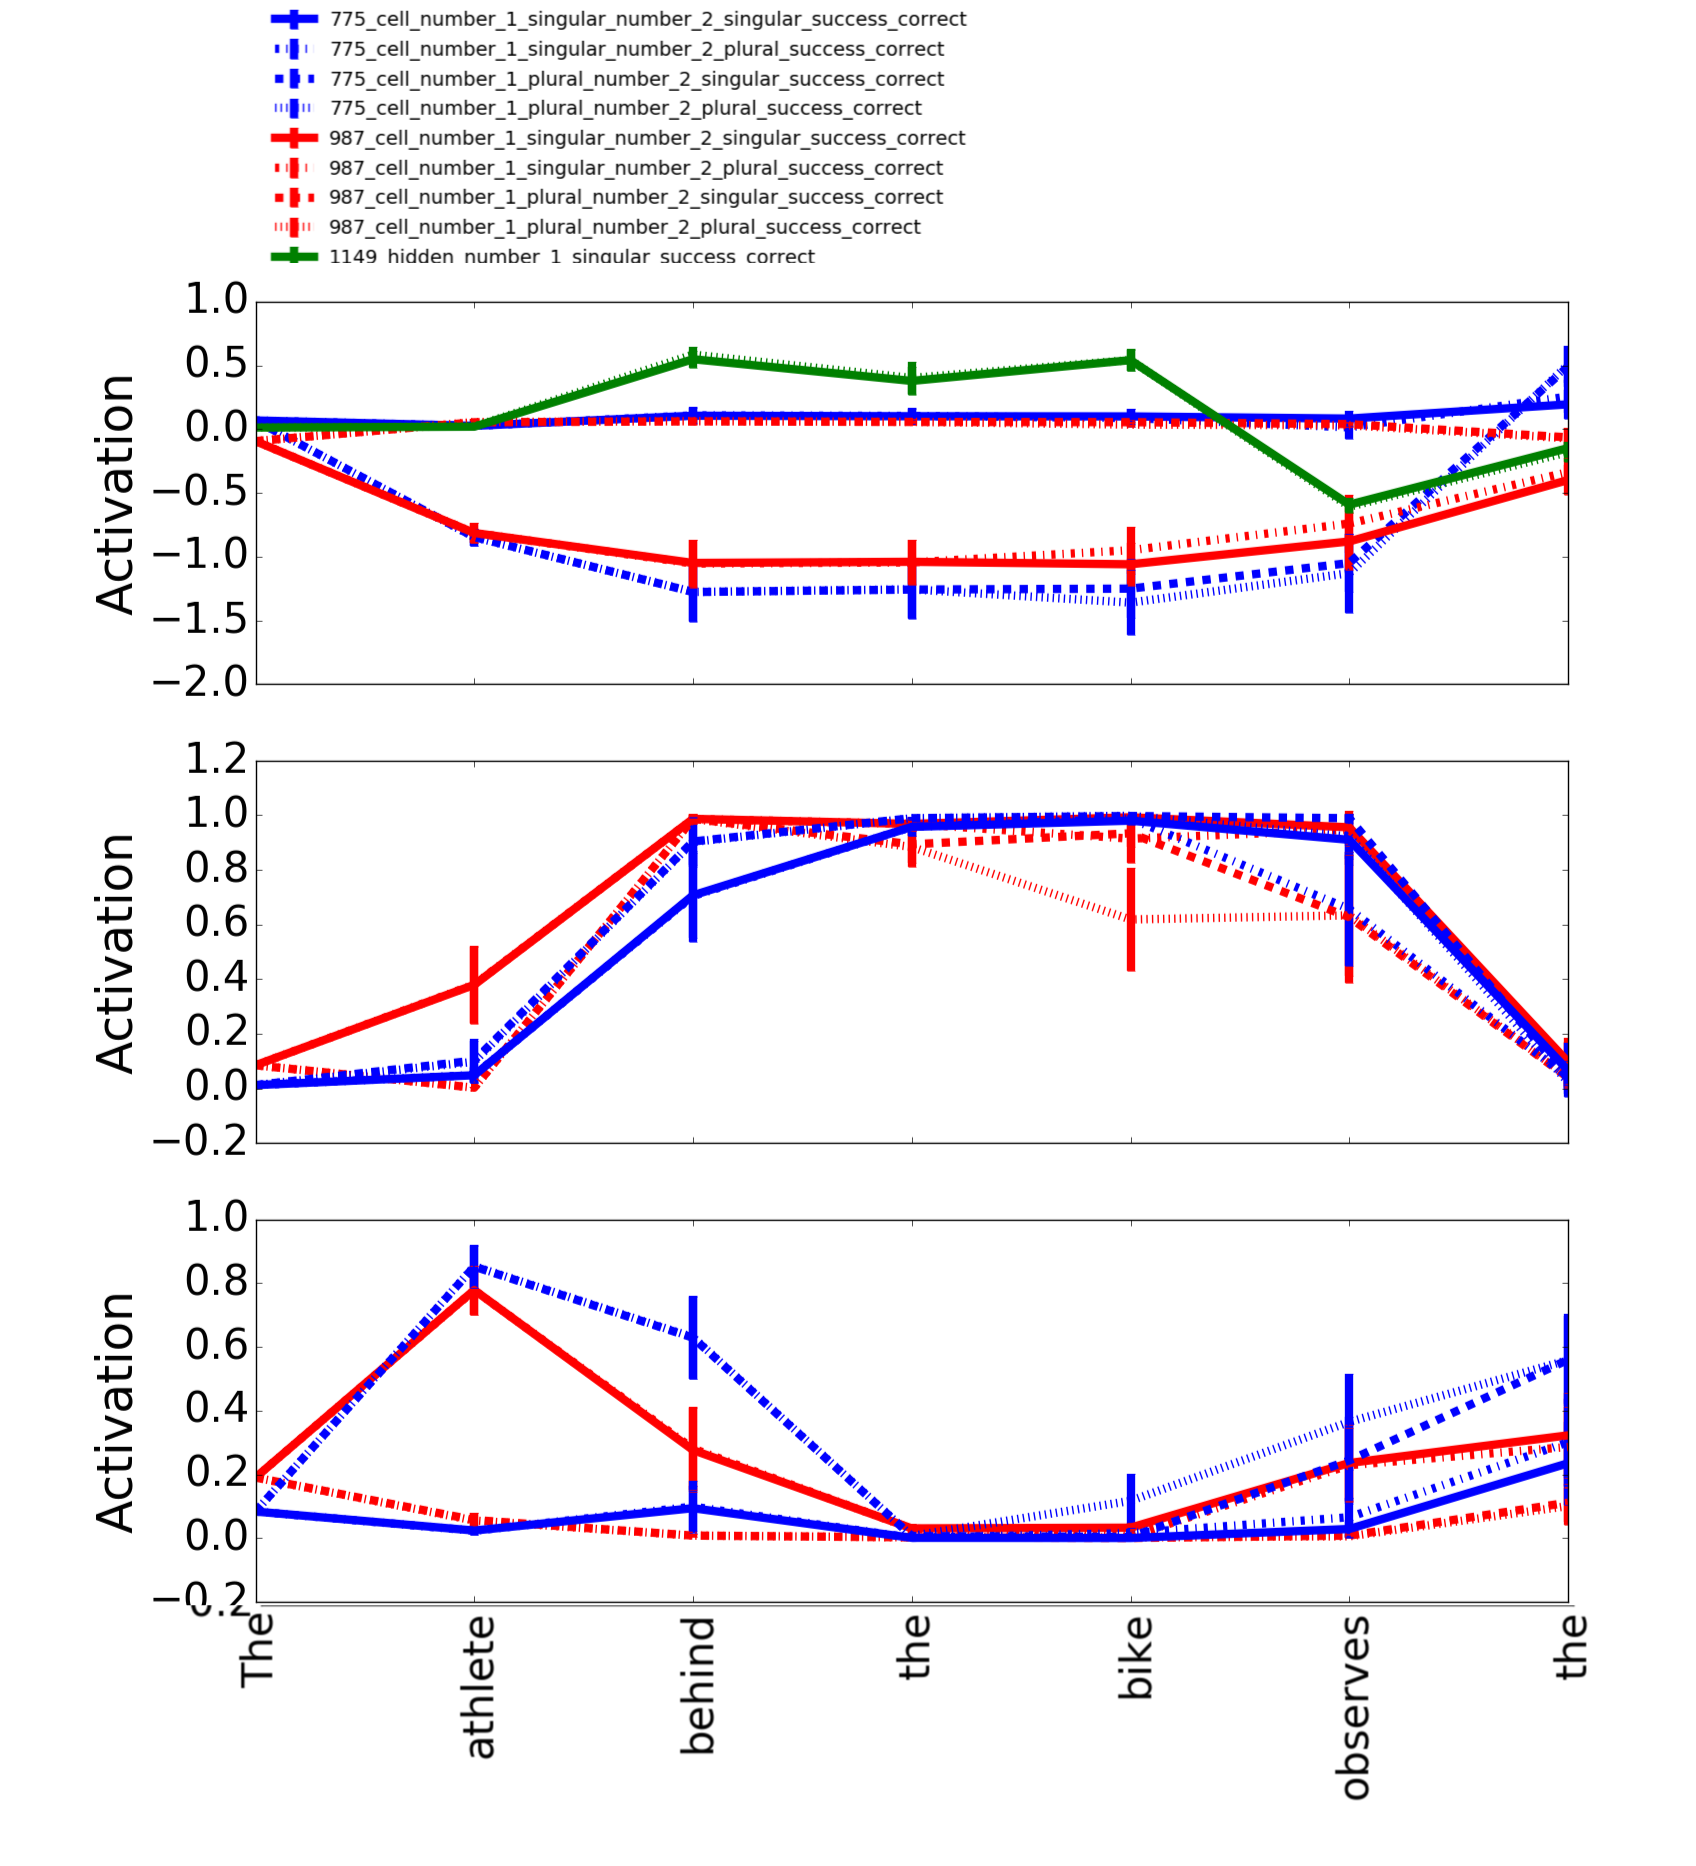
\includegraphics[width=\linewidth]{Figures/Figure2_number_units.png}
\caption{Cell and gate activations during processing of a sentence with a prepositional phrase between subject and verb. (A) Cell activity $C_t$ for the two number units 775 and 987 and output activity $h_t$ for the syntax unit 1149, for all four combinations of grammatical numbers of the two nouns. Note that the cell activity of units 775/987 is non-zero only when the first noun is plural/singular, respectively. (B) Corresponding forget-gate activity for the same number units. Note that gate activity is indifferent of the grammatical number of both nouns and that its value is close to one during the PP until after the verb. (C) Input-gate activity of the same units. Note that the gate value of unit 775/987 spikes around the first noun only when it is plural/singular.}
\end{figure}

\lipsum[1]

\begin{figure}
\centering
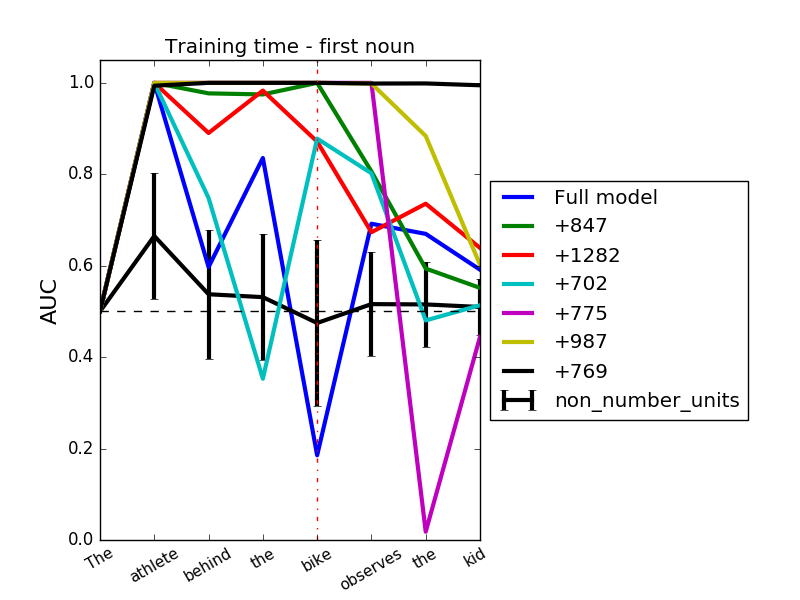
\includegraphics[width=\linewidth]{Figures/Figure3_number_units_GAT.png}
\caption{Generalization across time. To test whether the grammatical number of the first noun can be decoded from units activity at different time points, a linear-SVM was trained on unit activations $h_t$ at the time step of the first noun and then evaluated on all other time points. Area Under of Curve (AUC) values are shown for several cases: decoding from all LSTM units (full-model, black), a single number unit (775, purple; 1282, red...), average across all non-number units (black, error-bars represent standard-deviation). Note that the decoding of first-noun number is significantly higher from number units compared to all other units ($p-value<0.$).}
\end{figure}

\lipsum[1]

\subsubsection{Predicting the verb form}
Output weights + PCA
\lipsum[1]

\begin{figure*}[t]
\centering
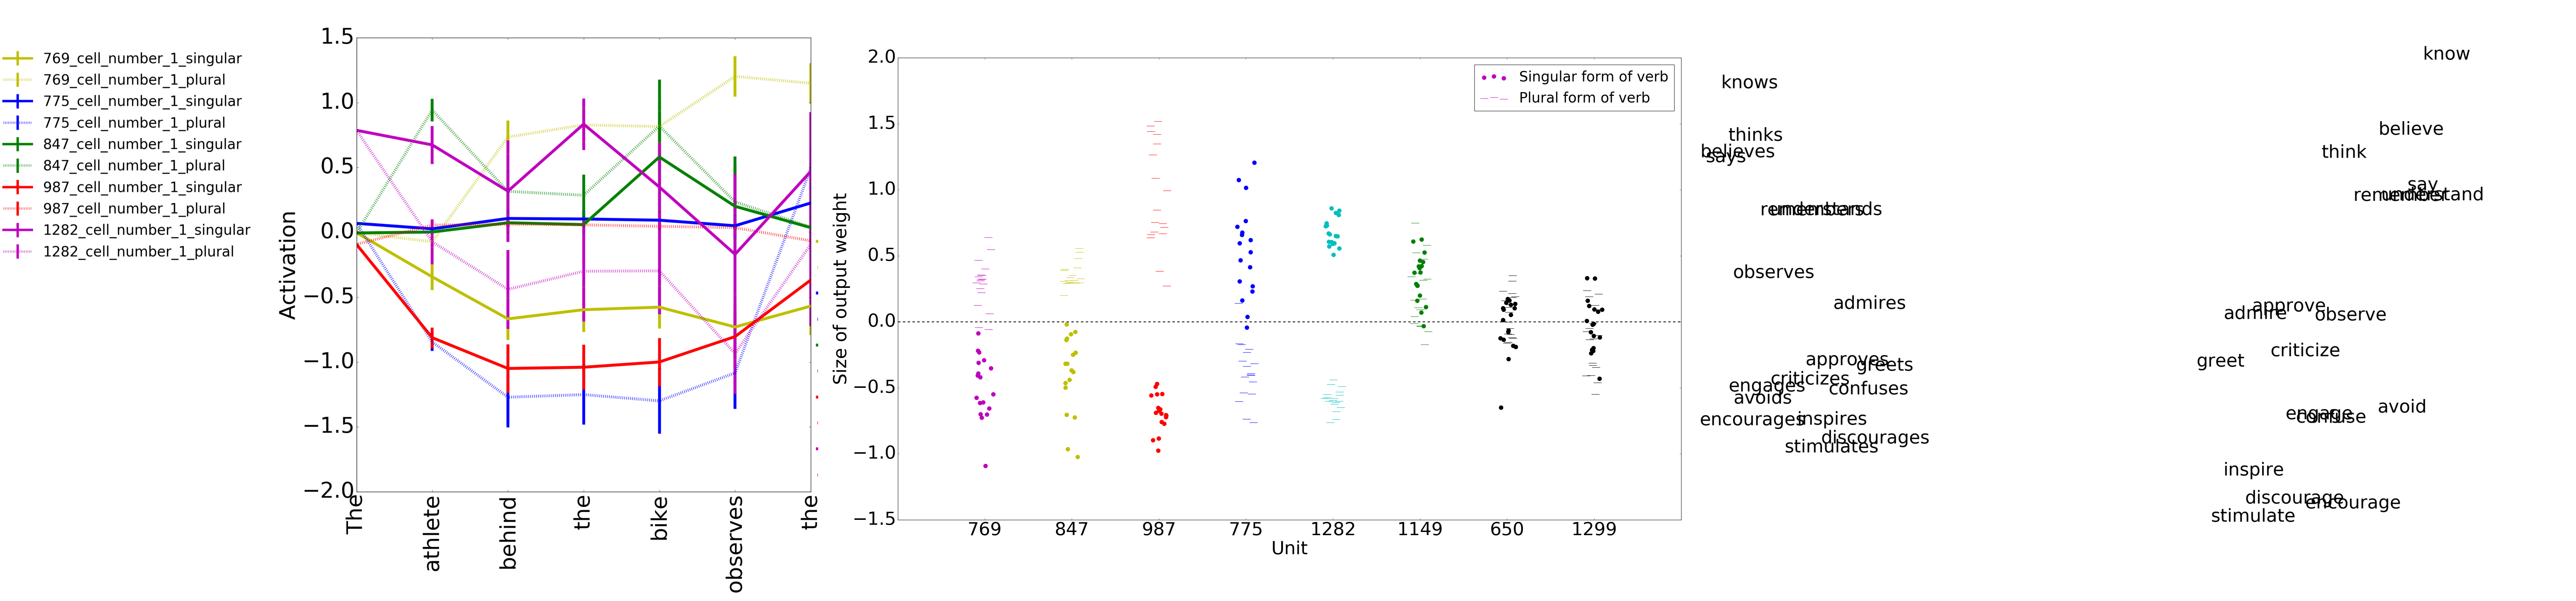
\includegraphics[width=\textwidth]{Figures/Figure4_output_weights.png}
\caption{Connectivity structure to output layer. (A) Output activity $h_t$ of all number units during the processing of a sentence with a PP between subject and verb. (B) Weight values from various units to output layer. Note that only for number units the output weights are clearly separated between singular and plural form of the verb, either positive or negative, compare to the syntax unit (1149) and two non-number units in the second layer. (C) Visualization of 18 verbs in their plural and singular forms (36 words in total) on the plane spanned by the two first principal components of their embeddings by the output weight matrix. A clear separation is observed between the singular and plural form along the first PC.}
\end{figure*}

\begin{figure}[b]
\centering
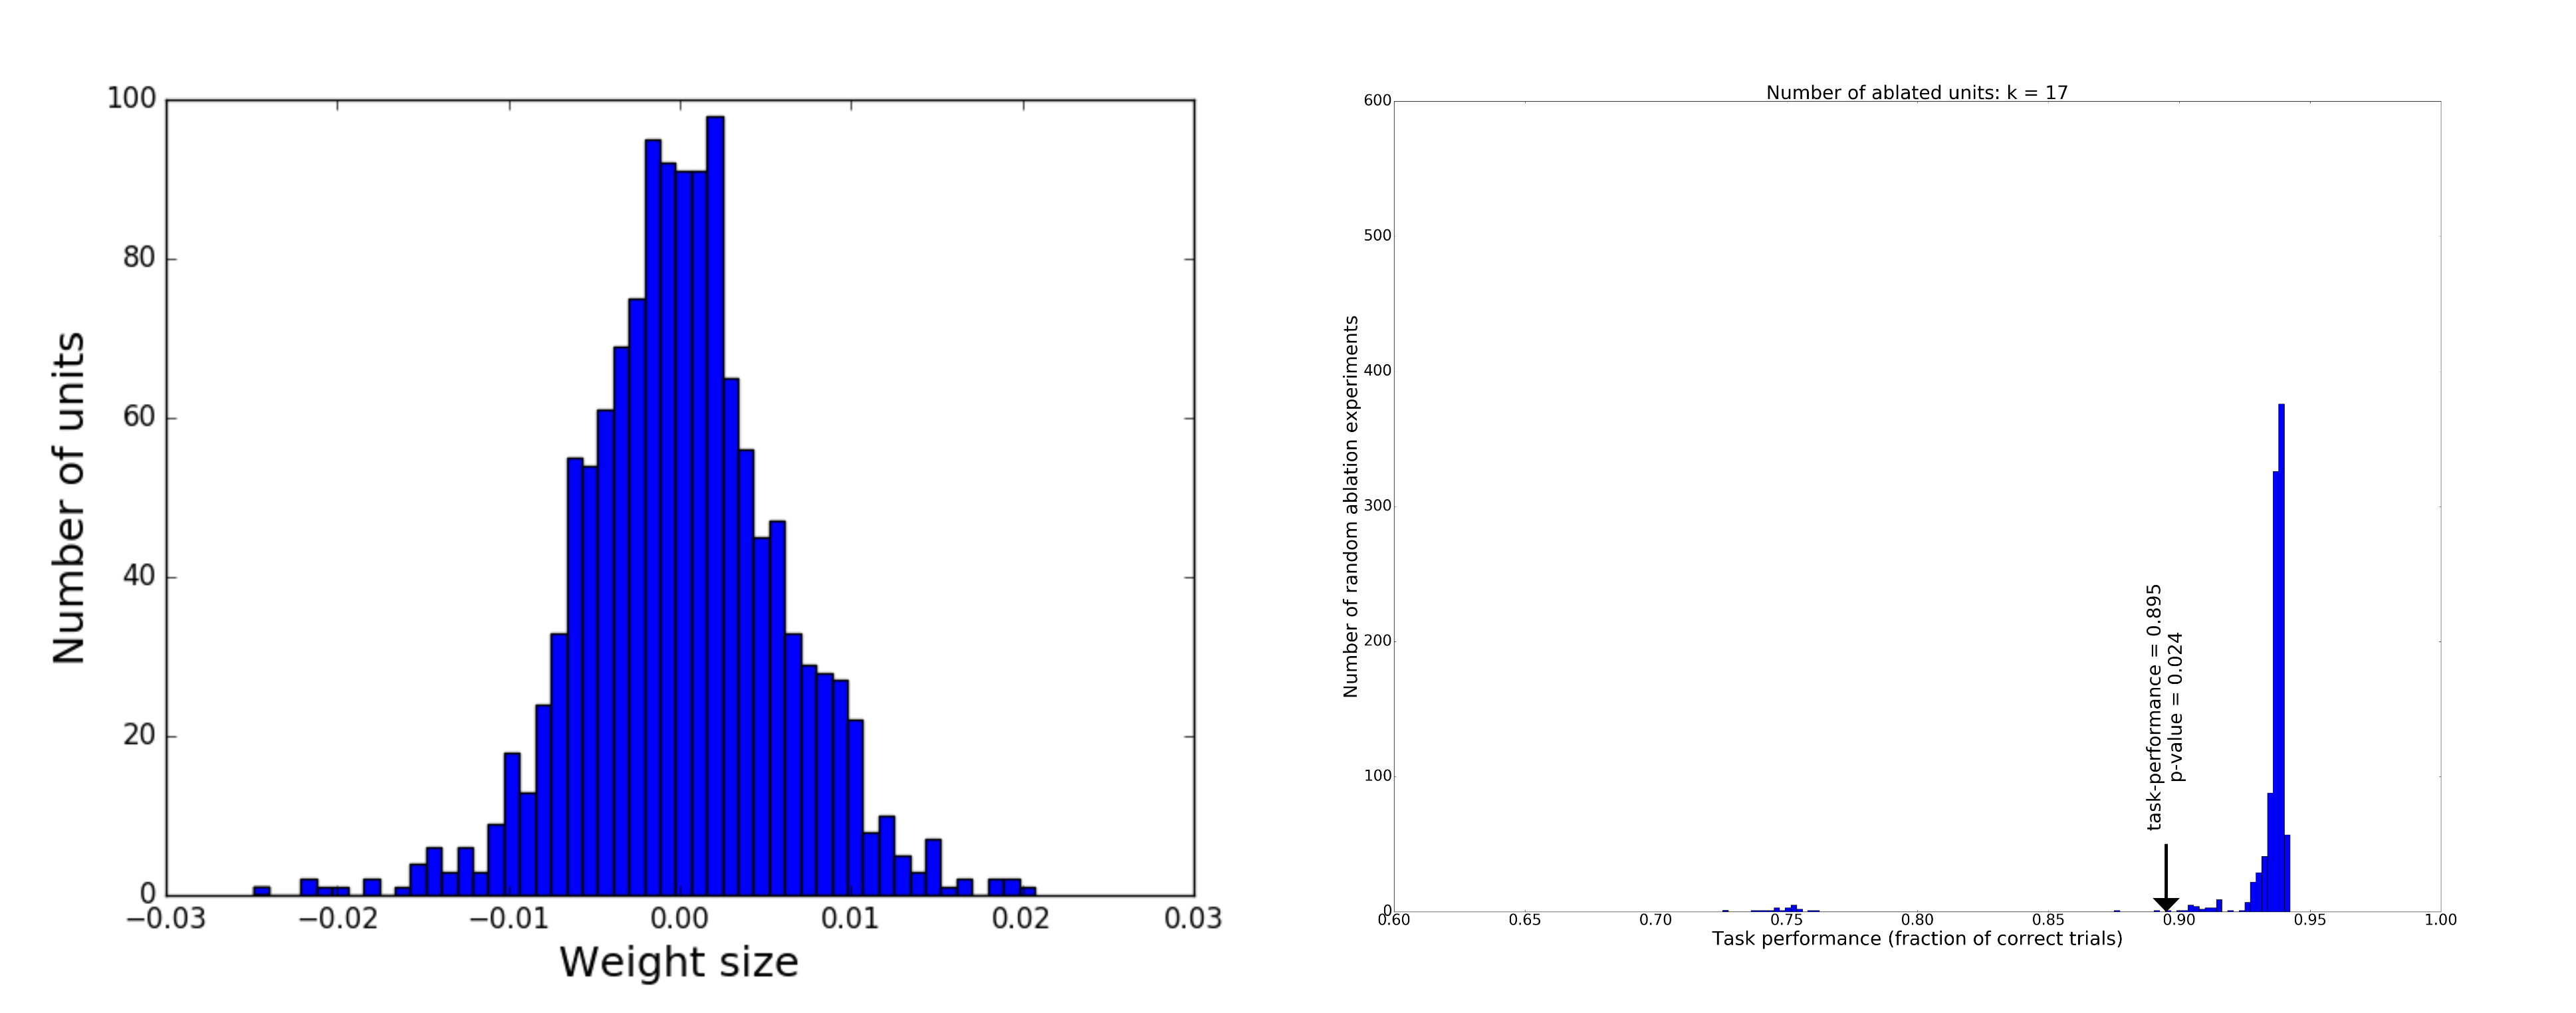
\includegraphics[width=\linewidth]{Figures/Figure6_regression.png}
\caption{(A) Distribution of the resulting weight values from the tree-depth regression model. Outlier weights were defined as having a value that is distant from the mean by more than three standard deviations (17 outlier weights in total - marked in red). (B) Task performance of 1000 models after ablating 17 random units (in blue) and based on the 17 outlier weights from the tree-depth regression model (black arrow). The reduction in performance due to outlier-weights ablation is statistically significant ($p-value < 0.05$) when compared to the null distribution generated by the random ablations.}
\end{figure}

